% !TeX spellcheck = cs_CZ
% options:
% thesis=B bachelor's thesis
% thesis=M master's thesis
% czech thesis in Czech language
% slovak thesis in Slovak language
% english thesis in English language
% hidelinks remove colour boxes around hyperlinks
\RequirePackage{color}
\definecolor{gr1}{RGB}{0,153,51}
\documentclass[thesis=M,czech]{FITthesis}[2012/06/26]


\usepackage[utf8]{inputenc} % LaTeX source encoded as UTF-8

\usepackage{graphicx} %graphics files inclusion
\usepackage{amsmath} %advanced maths
\usepackage{amssymb} %additional math symbols
\usepackage{rotating}

\usepackage{dirtree} %directory tree visualisation
% % list of acronyms
% \usepackage[acronym,nonumberlist,toc,numberedsection=autolabel]{glossaries}
% \iflanguage{czech}{\renewcommand*{\acronymname}{Seznam pou{\v z}it{\' y}ch zkratek}}{}
% \makeglossaries
 

\newcommand{\tg}{\mathop{\mathrm{tg}}} %cesky tangens
\newcommand{\cotg}{\mathop{\mathrm{cotg}}} %cesky cotangens

% % % % % % % % % % % % % % % % % % % % % % % % % % % % % % 
% ODTUD DAL VSE ZMENTE
% % % % % % % % % % % % % % % % % % % % % % % % % % % % % % 

\department{Katedra geomatiky     }
\acknowledgements{Studijní program Geodézie a kartografie}

\title{Název}
\authorGN{Petra} %(křestní) jméno (jména) autora
\authorFN{Pasovská} %příjmení autora
\authorWithDegrees{Bc. Petra Pasovská} %jméno autora včetně současných akademických titulů
\supervisor{Ing. Tomáš Janata, Ph.D.}
\acknowledgements{Děkuji Ing. Tomáši Janatovi, Ph.D., za odborné vedení práce a cenné rady, které mi pomohly tuto práci zkompletovat. Velké díky také patří mé rodině a přátelům, kteří mi byli po dobu zpracování velkou oporou.}
\abstractCS{Abstrakt CZ}
\abstractEN{Abstrakt EN}
\placeForDeclarationOfAuthenticity{V~Praze}
\declarationOfAuthenticityOption{1} %volba Prohlášení (číslo 1-6)
\keywordsCS{klicova slova \newpage}
\keywordsEN{keywords}

\begin{document}

% \newacronym{CVUT}{{\v C}VUT}{{\v C}esk{\' e} vysok{\' e} u{\v c}en{\' i} technick{\' e} v Praze}
% \newacronym{FSv}{FSv}{Fakulta stavebn{\' i}}

\begin{introduction}
Úvod


\end{introduction}

\chapter{Rešerše literatury}
Tato práce se dotýká tří hlavních témat - hydrologie, modelování a obecně řeky Otavy. Za tímto účelem byla provedena rešerše literatury na všechny tři hlavní oblasti. \\
\\
Knih týkajících se hydrologie je mnoho. Jednotlivé pojmy a jejich vysvětlení se však již ustálily. 


\chapter{Hydrologie}

Hydrologie je věda, která se zabývá zkoumáním zákonitostí výskytu, oběhu, časového a prostorového rozložení zásob vody na Zemi, jejího vzájemného působení s biotickými a abiotickými faktory s ohledem na její fyzikální, chemické a biologické vlastnosti. \cite{definiceHydro} 


S hydrologií úzce souvisí i hydrogeografie, což je jedna z dílčích fyzickogeografických věd zabývající se vztahem mezi vodními útvary na pevnině a ostatními krajinotvornými prvky. Od hydrologie se liší tím, že že používá převážně geografické metody při studiu hydrologických jevů a procesů. \cite{FGkniha}


Hydrologii lze rozdělit podle dvou hlavních kritérií - dle pracovních metod a dle prostředí. Podle pracovních metod se rozděluje na hydrometrii a hydrografii. Hydrometrie zahrnuje měření mechanických, fyzikálních, chemických a biologických jevů ve vodních systémech, hydrografie popisuje hydrologické jevy, hydrologické prostředí, vlastnosti vodních systémů, třídění zpracování a klasifikaci získaných informací. Podle prostředí se rozděluje na hydrologii pevnin (ta lze následně rozdělit na hydrologii atmosféry, řek, jezer, bažin, podzemních vod a ledovců) a hydrologii oceánů. \cite{hydro_net}

Součástí hydrologie je několik vědních oborů. Za zmínku stojí například hydrometeorologie, hydroklimatologie či hydrogeologie. Přesto není do hydrologie začleněna oceánografie a meteorologie, neboť voda je jen jedním ze zkoumaných aspektů. Hydrologie byla řadu let analyzována v rámci geografie. Oddělila se až v 19. století jako samostatná vědní disciplína hydrologie. 

Počátky studia vody na Zemi však sahají do roku 3000 př. n. l. V té době ve starověkém Egyptě byla sledována hladina Nilu na tzv. nilometrech.\footnote{Nilometr je moderní označení pro stavbu ve starověkém Egyptě pro měření výšky nilských záplav. Mají podobu dlouhé sestupné chodby nebo studny a většinou jsou propojeny s hladinou Nilu. Výška byla určována v loktech.} Podobná pozorování probíhala i v Mezopotámii na řece Eufrat a Tigris nebo v Číně. Vodou se zabývali i řečtí filozofové, zejména Thales z Milétu, Platón či Aristoteles. 


Ústředním tématem této práce je řeka Otava. Z hydrologického hlediska tedy budou blíže prozkoumány jen pojmy a analýza týkající se řek.


\begin{figure}[h!]
	\centering
	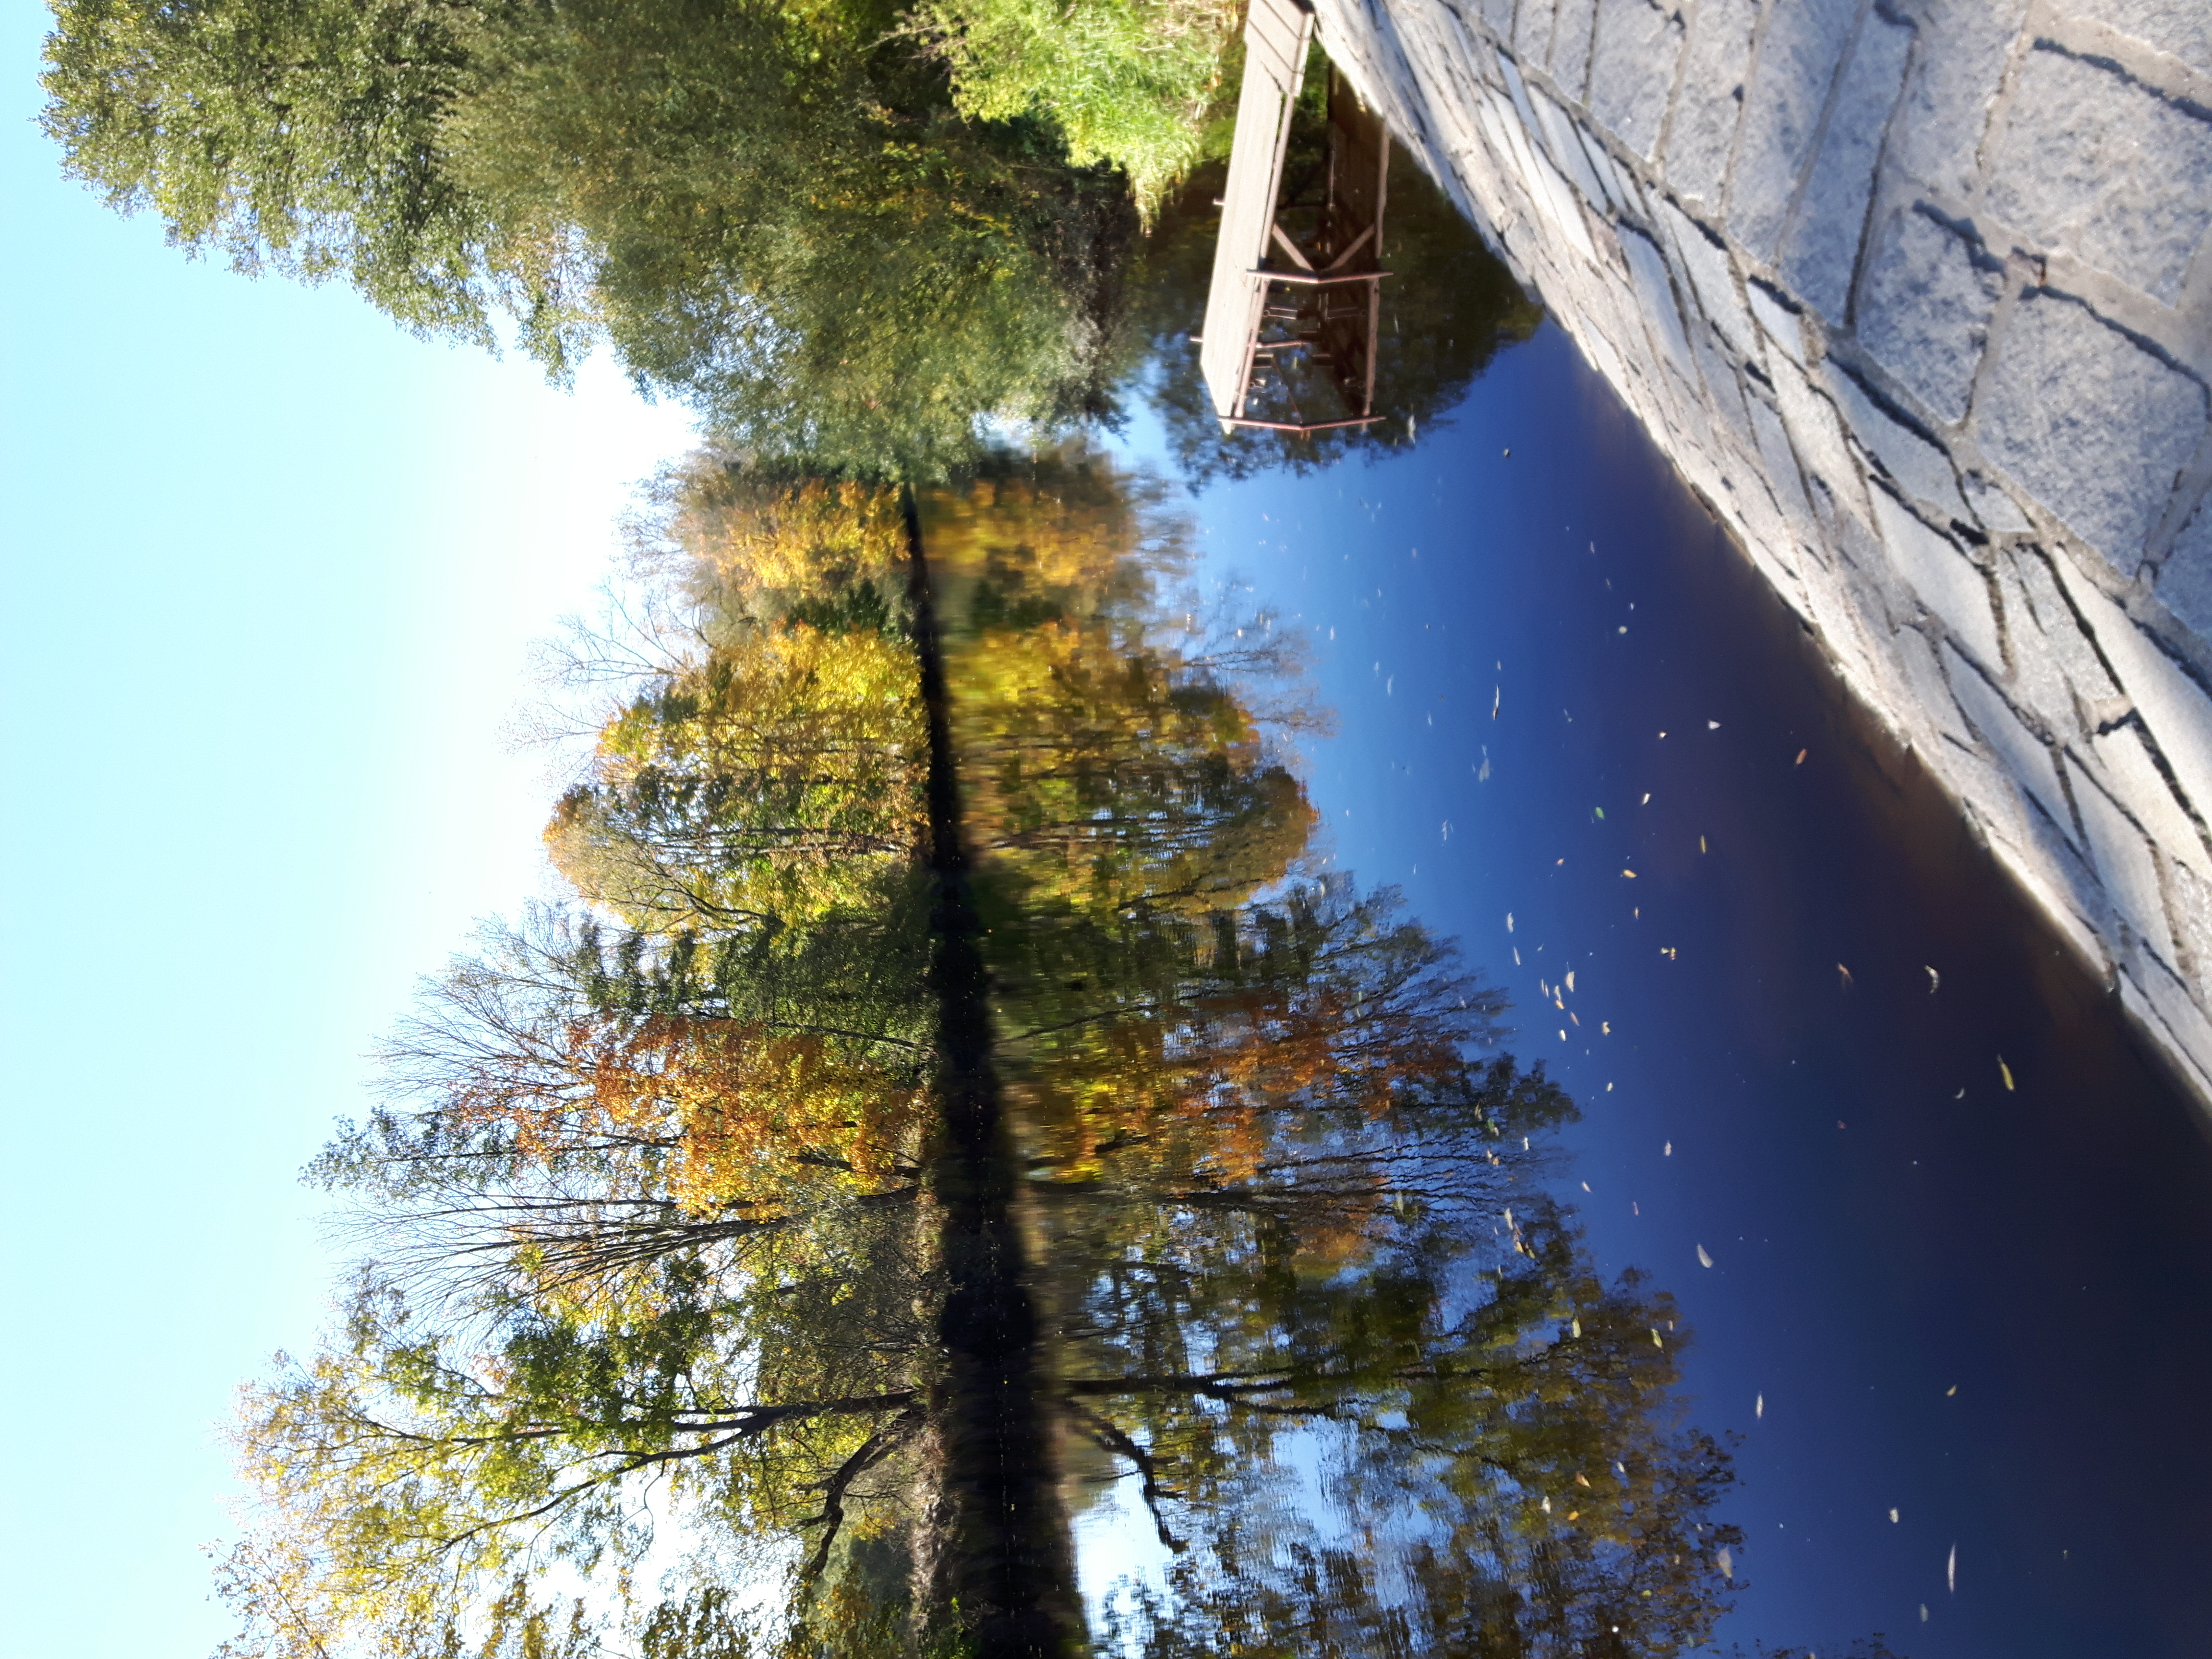
\includegraphics[width=10cm, angle =270]{pics/ot1.jpg}
	\caption{Otava na Podskalí ve Strakonicích na podzim}
	\label{obrazek:ot1}
\end{figure}


\section{Vysvětletní základních termínů (pojmů??)}
Při hydrologické analýze jsou používány základní hydrologické termíny. Ty jsou zde stručně popsány a vysvětleny, aby 

\begin{description}
\item[pramen] text
\item[říční tok] text
\item[říční síť] text
\item[hustota říční sítě] text
\item[povodí] text
\item[rozvodí] text
\item[úmoří] text
\item[přítok] text
\item[ústí] text
\item[zátopové území] text
\end{description}



\section{Hydrologická analýza}






\chapter{Kartografické podklady}




\chapter{Kulturní a historické informace o oblasti}


\chapter{Modelování}

\chapter{Diskuze}



\begin{conclusion}
Závěr
\end{conclusion}

\bibliographystyle{csn690}
\bibliography{mybibliographyfile}

\appendix

\chapter{Seznam použitých zkratek}
% \printglossaries
\begin{description}
	\item[GIS] Geografický informační systém

\end{description}



\chapter{Obsah přiloženého CD}

\begin{figure}
	\dirtree{%
		.1 readme.txt\DTcomment{stručný popis obsahu CD}.
		.1 grafy\DTcomment{složka obsahující výsledné grafy}.
		.1 rastry\DTcomment{složka obsahující testované rastry}.
		.1 rozklad.m\DTcomment{skript na výpočet rozkladu RGB barev}.
		.1 LaTex\DTcomment{zdrojová forma práce ve formátu \LaTeX{}}.	
		.1 text\DTcomment{text práce}.
		.2 BP\_Pasovska\_Petra\_2017\DTcomment{text práce v PDF}.	
	}
\end{figure}

\end{document}